% !TeX program = pdflatex
\documentclass[tikz,border=8pt]{standalone}
\usepackage{tikz}\usetikzlibrary{angles,quotes,calc}
\definecolor{FigureBlue}{HTML}{2563EB}\definecolor{FigureOrange}{HTML}{EA580C}
\begin{document}
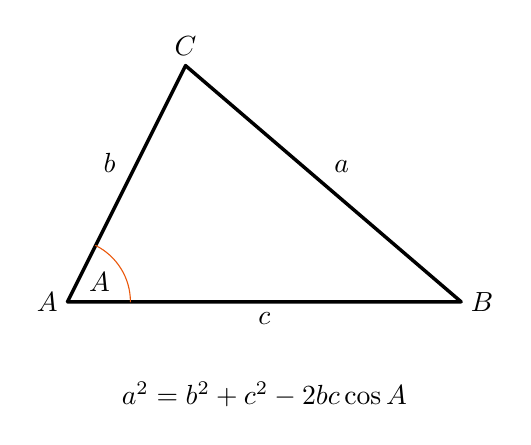
\begin{tikzpicture}[line cap=round,line join=round]
  \coordinate (A) at (0,0); \coordinate (B) at (5,0); \coordinate (C) at (1.5,3);
  \draw[line width=1.25pt] (A)--node[below] {$c$}(B)--node[above right] {$a$}(C)--node[above left] {$b$}(A);
  \pic[draw=FigureOrange,angle radius=8mm,"$A$"] {angle=B--A--C};
  \node[left] at (A) {$A$}; \node[right] at (B) {$B$}; \node[above] at (C) {$C$};
  \node[below=9mm] at ($(A)!.5!(B)$) {$a^2=b^2+c^2-2bc\cos A$};
\end{tikzpicture}
\end{document}
